\chapter{TỔNG QUAN VỀ MACHINE LEARNING}
\section{Giới thiệu Machine Learning}
Machine learning (ML) hay máy học là một nhánh của trí tuệ nhân tạo (AI) và khoa học máy tính, tập trung vào việc sử dụng dữ liệu và thuật toán để bắt chước cách con người học, dần dần cải thiện độ chính xác của nó.\\
Học máy là một thành phần quan trọng của lĩnh vực khoa học dữ liệu đang phát triển. Là ngành khoa học giúp máy tính dự đoán được các dữ liệu mới từ các dữ liệu đã biết thông qua các giải thuật học máy. Thông qua việc sử dụng các phương pháp thống kê, các thuật toán được đào tạo để đưa ra các phân loại hoặc dự đoán và khám phá những hiểu biết quan trọng trong các dự án khai thác dữ liệu. Những thông tin chi tiết này sau đó thúc đẩy việc đưa ra quyết định trong các ứng dụng và doanh nghiệp, tác động lý tưởng đến các chỉ số tăng trưởng chính.
\section{Hoạt động của Machine Learning}
\subsection{Quy trình ra quyết định}
Nói chung, các thuật toán học máy được sử dụng để đưa ra dự đoán hoặc phân loại. Dựa trên một số dữ liệu đầu vào, có thể được gắn nhãn hoặc không được gắn nhãn, thuật toán của bạn sẽ đưa ra ước tính về một mẫu trong dữ liệu. Các thuật toán học máy phải đủ tốt để phù hợp với yêu cầu của bài toán và phù hợp với bộ dữ liệu mẫu. Tức là, muốn ra được một quyết định đáng tin cậy, cần phải chứng minh được thuật toán có đầu ra phù hợp để đưa ra quyết định.\\
Với bộ dữa liệu đầu vào đã được xử lí thô, một mô hình học máy phải học được các tri thức ẩn bên trong bộ dữ liệu, bằng việc học nhiều lần, mô hình ngày càng cải thiện tốt hơn và độ chính xác cao hơn, các quyết định được đưa ra đảm bảo độ tin cậy.
\subsection{Hàm lỗi và tham số mô hình}
Các mô hình Machine Learning - học máy khi được đào tạo trên bộ dữ liệu mẫu sẽ học được các bộ tham số được gọi là tham số mô hình (Model parameter). Mỗi mô hình sẽ có các tham số riêng phù hợp với từng bộ dữ liệu, một bộ tham số mô hình tốt phải đảm bảo mô hình có dự đoán chính xác cao, là kết quả tối ưu của bài toán.\\
Bằng việc đào tạo mô hình trên bộ dữ liệu mẫu, ta tiến dần tới một tham số tối ưu cho mô hình, nhằm cải thiện các phép đánh giá đạt kết quả tốt nhất. Thuật toán trong các mô hình cũng thường là các bài toán tối ưu, và việc đi tìm nghiệm tối ưu cũng giống với việc đi tìm tham số mô hình tối ưu đủ tốt cho việc dự đoán.\\
Trong các bài toán Machine Learning, để thực hiện đánh giá và cải thiện kết quả mô hình, ta biết đến với khái niệm hàm lỗi (Loss function) hay còn được gọi là hàm mất mát tương tự với hàm mục tiêu trong bài toán tối ưu. Công việc của đào tạo mô hình là tìm ra bộ tham số làm cho hàm lỗi đạt giá trị lỗi nhỏ nhất, tức là bài toán tối ưu $min$. Và như vậy giải bài toán ML cũng chính là giải bài toán tối ưu với mục đích tối thiểu hàm mục tiêu.\\
Hàm mất mát $L(\theta)$ với bài toán tối ưu, tìm tham số $\theta$ tối ưu hàm lỗi:
\begin{center}
\begin{equation*}
    \theta^*  = \mathop {\arg \min }\limits_\theta  L(\theta )
\end{equation*}    
\end{center}
Tham số tối ưu của mô hình là $\theta^*$.

\subsection{Quy trình tối ưu hóa}
Nếu mô hình có thể phù hợp hơn với các điểm dữ liệu trong tập huấn luyện, thì tham số được điều chỉnh để giảm sự khác biệt giữa mẫu đã biết và ước tính mô hình. Thuật toán sẽ lặp lại quá trình “đánh giá và tối ưu hóa”, cập nhật các trọng số một cách tự động cho đến khi đạt đến ngưỡng độ chính xác.\\
Thuật toán sử dụng vòng lặp cho mô hình học nhiều lần trên bộ dữ liệu mẫu từ đó cập nhật tham số mô hình.\\ Việc điều chỉnh các tham số qua các lần lặp dựa trên các thuật toán tối ưu có thể kể đến như Gradient descent. Sau mỗi lần lặp, tham số sẽ được điều chỉnh để di chuyển đến nghiệm tối ưu. Trong quá trình tối ưu hóa, các tham số của ta có thể rơi vào nhiều  các nghiệm cực tiểu địa phương, vì đó ta có thể lựa chọn tham số phù hợp với yêu cầu đặt ra để có được đánh giá kết quả khả quan.
\section{Tập dữ liệu}
Câu hỏi đặt ra cho các mô hình học máy là nó sẽ làm việc trên những tập dữ liệu như thế nào. Các nhiệm vụ trong machine learning được mô tả thông qua việc một hệ thống xử lý một điểm dữ liệu đầu vào ra làm sao.\\
Một điểm dữ liệu có thể là một bức ảnh, một đoạn âm thanh, một văn bản, hoặc
một tập các hành vi của người dùng trên Internet. Để chương trình máy tính có thể học được, các điểm dữ liệu thường được đưa về dạng tập hợp các con số mà mỗi số được gọi là một đặc trưng (feature).\\
Do đó, việc biến đổi dữ liệu đầu vào cần được thực hiện một cách phù hợp với khả năng xử lý của từng thuật toán. Điều này không những làm tăng hiệu quả của thuật toán mà còn làm mô hình xử lý nhanh hơn. Việc hiểu biết sâu sắc về các loại dữ liệu khác nhau là một yêu cầu thiết yếu để thực hiện được các quá trình phân tích, khám phá dữ liệu trong machine learning.\\
Trong Machine learning, tập dữ liệu thường được biểu diễn dưới dạng tập hợp của các thuộc tính, một tập dữ liệu có nhiều thuộc tính thì dữ liệu càng đa dạng và có thể mang lại nhiều giá trị tri thức bên trong nó.\\
Dữ liệu có thể được chia thành 2 dạng chính là:
\begin{itemize}
    \item Dữ liệu dạng định tính (Categorical Data): Dữ liệu định tính được biểu diễn dưới dạng các chuỗi ký tự cho phép xác định các tính chất, đặc tính hoặc trạng thái của dữ liệu ví dụ như: cao, thấp, gầy, béo.
    \item Dữ liệu dạng định lượng (Numerical Data): Được biểu diễn thành dạng các số nguyên và thực cho phép xác định cường độ của các thuộc tính ví dụ 170cm, 150cm, 50kg hay 60kg.
\end{itemize}
\subsection{Các loại dữ liệu trong ML}
\subsubsection{Dữ liệu dạng bản ghi (Record)}
Dữ liệu dạng bản ghi là loại dữ liệu mà mỗi điểm dữ liệu bao gồm nhiều thuộc tính, tập hợp lại thành một bản ghi, các bản ghi có các thuộc tính giống nhau được ghép lại biểu diễn dưới dạng bảng. Một bảng dữ liệu với các cột là các thuộc tính và các hàng là các bản ghi, mỗi bản ghi hay còn gọi là một điểm dữ liệu.
\subsubsection{Dữ liệu dạng đồ thị (Graph)}
Dữ liệu dạng đồ thị là dạng dữ liệu phức tạp trong đó các đối tượng dữ liệu là các node trong đồ thị và các node có mối liên hệ tương quan với nhau. Việc biểu diễn các tương quan này khiến cho số chiều dữ liệu cực lớn và phức tạp. Đại diện phổ biến nhất của dữ liệu dạng này là: tương quan mạng xã hội, trong đó mỗi người là một node của đồ thị, mối tương quan là quan hệ bạn bè giữa các người dùng. Các tập dữ liệu dạng này thường phù hợp với bài toán khai phá phương tiện truyền thông xã hội (Social Media Mining).
\subsubsection{Dữ liệu dạng chuỗi (Sequential)}
Dữ liệu dạng chuỗi là dạng dữ liệu mà các điểm dữ liệu được sắp xếp thành chuỗi theo thứ tự, có nghĩa là thứ tự xuất hiện có vai trò và ý nghĩa nhất định trong tập dữ liệu. Một số dạng phổ biến như dữ liệu chuỗi thời gian, dữ liệu dạng văn bản, dữ liệu dạng video,...
\begin{itemize}
    \item Dữ liệu chuỗi thời gian: Được định nghĩa là những điểm dữ liệu đã được đánh chỉ mục theo thời gian và có khoảng cách đều nhau giữa những quan sát liên tiếp. Mỗi điểm dữ liệu gắn với một giá trị thời gian giúp chúng ta có thể quan sát xu hướng biến đổi theo thời gian của dữ liệu nhằm đưa ra dự đoán.
    \item Dữ liệu chuỗi văn bản: Dạng dữ liệu là văn bản các từ, các từ theo thứ tự xuất hiện khác nhau có thể làm thay đổi ý nghĩa đoạn văn bản. Dữ liệu dạng này thường sử dụng cho các bài toán về xử lí ngôn ngữ tự nhiên.
    \item Dữ liệu dạng video: Dữ liệu dạng các hình ảnh, khung hình liên tiếp của một video được xuất hiện. Ở đây khi cắt từng khung hình của video chính là một điểm dữ liệu đầu vào của mô hình, cắt các khung hình liên tiếp nhau ta được một dạng dữ liệu chuỗi. Dữ liệu dạng này thường được sử dụng cho các bài toán về thị giác máy tính trong lĩnh vực học sâu (Deep Learning).
\end{itemize}
\subsection{Cách chia tập dữ liệu}
Khi đã có tập dữ liệu về bài toán, ta cần phải chia dữ liệu thành các tập nhỏ hơn để thực hiện việc huấn luyện mô hình, và để đánh giá mô hình. Khi đó tập dữ liệu thường có 3 tập nhỏ: Training set, Validation set, Test set.
\subsubsection{Tập huấn luyện (Training set)}
Là tập dữ liệu được sử dụng huấn luyện mô hình, mô hình sẽ học các tham số trên tập dữ liệu này. Tập Train thường là tập chiếm phần lớn dữ liệu, giúp cho mô hình học tốt hơn.
\subsubsection{Tập xác thực (Validation set)}
Tập Validation cung cấp các đánh giá công bằng về sự phù hợp của mô hình trên tập dữ liệu huấn luyện trong quá trình huấn luyện. Validation set như một tập kết hợp: nó vừa là dữ liệu huấn luyện được sử dụng để thử nghiệm, nhưng không phải là một phần của quá trình huấn luyện cấp thấp cũng không phải là một phần của thử nghiệm cuối cùng. Nó là một bước trung gian cho phép lựa chọn mô hình phù hợp. Ta dựa vào kết quả đánh giá trên tập Validation để điều chỉnh các tham số mô hình, điều chỉnh cách hoạt động mô hình để cải thiện chúng, nhằm đạt kết quả tốt hơn.
\subsubsection{Tập thử nghiệm (Test set)}
Khi huấn luyện xong mô hình trên tập Training set, ta có được bộ tham số đủ tốt trên bộ dữ liệu train và xác thực trên tập Validation có thể mô hình đã học tập tốt, nhưng chúng ta vẫn cần kiểm tra lần cuối chúng trên tập Test để xem chúng có thực sự tốt. Tập Test phải có cùng một phân phối dữ liệu với tập Validation để cho quá trình kiểm tra được chính xác nhất. Khi mô hình của chúng ta có kết quả tốt trên tập Validation nhưng kết quả ở tập Test lại không như thế, tức chúng ta cần thực hiện lại huấn luyện mô hình.

\section{Các phương pháp học máy - ML}
\subsection{Học máy có giám sát - Supervised learning}
Một thuật toán được gọi là học có giám sát khi mô hình học trên tập dữ liệu có gán nhãn để đào tạo các thuật toán phân loại dữ liệu hoặc dự đoán kết quả một cách chính xác. Tức là máy học mối quan hệ giữa đầu vào và đầu ra chính xác được gọi là một cặp (input,output) trong tập huấn luyện. Điều này đòi hỏi thuật toán học tập phải tổng quát hóa từ dữ liệu đào tạo đến các tình huống chưa thấy một cách "hợp lý". Đây là một phương pháp học máy phổ biến trong Machine learning.\\
Một cách dễ hiểu, ta có một tập biến đầu vào $X = (x_1,x_2,...,x_N)$ và tập nhãn (label) tương ứng là $Y = (y_1,y_2,...,y_N)$,$x_i,y_i$ là các vector khi đó mỗi cặp $(x_i,y_i) $ với $i\in N$ được gọi là một điểm dữ liệu huấn luyện. Thuật toán học máy sẽ học một hàm $f(x)$ để ánh xạ từ $X$ vào $Y$:
\begin{center}
\begin{equation*}
    {y_i} \approx f({x_i}),i \in N
\end{equation*}
\end{center}
Khi đó thuật toán của chúng ta đang học xấp xỉ hàm $f$ tốt nhất để khi có dữ liệu với vào thì ta có thể dùng để dự đoán được nhãn của nó.\\
\textbf{Ví dụ:} Một bài toán về nhận dạng chữ số viết tay, tập dữ liệu của ta là hình ảnh về các con số viết tay, và nhãn chính xác của nó. Ta sẽ cho dữ liệu vào cho mô hình học, sau đó, lấy một bức ảnh số viết tay mới mà mô hình chưa từng nhìn thấy, và cho nó dự đoán nhãn.\\
Học có giám sát có thể được tách thành hai vấn đề cơ bản sau:
\begin{itemize}
    \item \textbf{Phân loại} sử dụng một thuật toán để chỉ định chính xác dữ liệu thử nghiệm thành các loại nhãn cụ thể. Nó nhận ra các thực thể cụ thể trong tập dữ liệu và cố gắng đưa ra kết luận về các thực thể đó nên được gắn nhãn hoặc định nghĩa. Các thuật toán phân loại phổ biến là bộ phân loại tuyến tính, máy vectơ hỗ trợ (SVM), cây quyết định, k-láng giềng gần nhất và rừng ngẫu nhiên, được mô tả chi tiết hơn bên dưới.
    \item \textbf{Hồi quy} được sử dụng để hiểu mối quan hệ giữa các biến phụ thuộc và độc lập. Nó thường được sử dụng để lập dự báo, chẳng hạn như doanh thu bán hàng cho một doanh nghiệp nhất định. Hồi quy tuyến tính , hồi quy logistical và hồi quy đa thức là các thuật toán hồi quy phổ biến.
\end{itemize}
Các thuật toán học tập có giám sát:
\subsubsection{Hồi quy tuyến tính}
Hồi quy tuyến tính được sử dụng để xác định mối quan hệ giữa một biến phụ thuộc và một hoặc nhiều biến độc lập và thường được sử dụng để đưa ra dự đoán về kết quả trong tương lai. Khi chỉ có một biến độc lập và một biến phụ thuộc, nó được gọi là hồi quy tuyến tính đơn giản. Khi số lượng các biến độc lập tăng lên, nó được gọi là hồi quy tuyến tính bội. Đối với mỗi loại hồi quy tuyến tính, nó tìm cách vẽ một đường phù hợp nhất, được tính bằng phương pháp bình phương cực tiểu. Tuy nhiên, không giống như các mô hình hồi quy khác, đường của mô hình hồi quy tuyến tính là đường thẳng khi được vẽ trên đồ thị. Thể hiện mỗi quan hệ tuyến tính giữa dữ liệu đầu vào và nhãn đầu ra.
\subsubsection{Hồi quy Logistic}
Trong khi hồi quy tuyến tính được tận dụng khi các biến phụ thuộc liên tục, thì hồi quy logisistic được chọn khi biến phụ thuộc có tính phân loại, nghĩa là chúng có đầu ra nhị phân, chẳng hạn như "đúng" và "sai" hoặc "có" và "không". Trong khi cả hai mô hình hồi quy đều tìm cách hiểu mối quan hệ giữa các đầu vào dữ liệu, thì hồi quy logistic chủ yếu được sử dụng để giải quyết các vấn đề phân loại nhị phân, chẳng hạn như nhận dạng thư rác. Trong hồi quy logistic ta có sử dụng hàm phi tuyến để phân loại.
\subsubsection{Naive Bayes}
Naive Bayes là một thuật toán phân loại được mô hình hoá dựa trên định lý Bayes trong xác suất thống kê, trong mô hình này ta sử dụng các xác xuất có điều kiện. Các đặc trưng đưa vào mô hình là độc lập với nhau. Tức là sự thay đổi giá trị của một đặc trưng không ảnh hưởng đến các đặc trưng còn lại và mỗi yếu tố dự đoán có ảnh hưởng như nhau đến kết quả đó.
\subsubsection{K-Nearest neighbor (K-NN)}
Đây là một thuật toán phân loại dựa trên các điểm dữ liệu tương đồng với nó nhất để phân loại chính xác nhãn dữ liệu. K-Nearest neighbor (KNN) là một thuật toán phi tham số phân loại các điểm dữ liệu dựa trên sự gần gũi và liên kết của chúng với các dữ liệu có sẵn khác. Đây còn gọi là bài toán lười học tập, vì mô hình của chúng ta không cần học tham số nào cả, chỉ dựa và những dữ liệu có sẵn để phân loại. Thuật toán này giả định rằng các điểm dữ liệu tương tự có thể được tìm thấy gần nhau. Kết quả là, nó tìm cách tính khoảng cách giữa các điểm dữ liệu, thường là thông qua khoảng cách Euclide, sau đó nó chỉ định một danh mục dựa trên danh mục hoặc mức trung bình thường xuyên nhất.
\subsubsection{Rừng ngẫu nhiên (Random forest)}
Rừng ngẫu nhiên là một thuật toán học máy có giám sát linh hoạt khác được sử dụng cho cả mục đích phân loại và hồi quy. "Rừng" tham chiếu đến một tập hợp các cây quyết định không tương quan, sau đó được hợp nhất với nhau để giảm phương sai và tạo ra các dự đoán dữ liệu chính xác hơn.
\subsection{Học máy không giám sát - Unsupervised learning}
Học không giám sát sử dụng các thuật toán học máy để phân tích và phân cụm các tập dữ liệu không được gắn nhãn. Các thuật toán này phát hiện ra các mẫu hoặc nhóm dữ liệu ẩn mà không cần sự can thiệp của con người. Mẫu dữ liệu sử dụng cho nhóm thuật toán này là dữ liệu không có nhãn, tức là ta chỉ biết đầu vào $X$ mà không biết label $Y$, mô hình học máy phải tự học những thông tin có trên tập dữ liệu mà không biết nhãn. Các mô hình phải có đủ khả năng để khám phá ra điểm tương đồng giữa những điểm dự liệu để thực hiện phân cụm dữ liệu hoặc phân tích thông tin.\\
Các bài toán phổ biến của học không giám sát:
\subsubsection{Phân cụm (Clustering)}
Phân cụm (clustering) là bài toán chia dữ liệu thành các cụm dựa trên
sự liên quan giữa các dữ liệu dựa trên những điểm tương đồng hoặc khác biệt của chúng. Trong bài toán này, dữ liệu huấn luyện không có nhãn (label), mô hình tự phân chia dữ liệu thành các cụm khác nhau.  Các thuật toán phân cụm được sử dụng để xử lý các đối tượng dữ liệu thô, chưa được phân loại thành các nhóm được biểu diễn bằng cấu trúc hoặc mẫu trong thông tin.\\
Các thuật toán phân cụm có thể được phân loại thành một số loại, cụ thể là phân cụm độc quyền (exclusive), phân cụm chồng chéo (overlapping), phân cụm phân cấp (hierarchical) và phân cụm xác suất (probabilistic).\\
Phân cụm độc quyền hay còn gọi là phân cụm cứng, khi mà mỗi điểm dữ liệu chỉ được phân vào một cụm duy nhất. Thuật toán phân cụm K-mean là một ví dụ, phân cụm K-mean là một ví dụ phổ biến của phương pháp phân cụm độc quyền trong đó các điểm dữ liệu được gán thành $K$ nhóm, trong đó $K$ đại diện cho số lượng các cụm dựa trên khoảng cách từ trung tâm của mỗi nhóm. Các điểm dữ liệu gần nhất với một trung tâm nhất định sẽ được nhóm lại trong cùng một cụm. \\
Phân cụm chồng chéo khác với phân cụm độc quyền ở chỗ nó cho phép các điểm dữ liệu thuộc về nhiều cụm với các cấp độ thành viên riêng biệt. Phân cụm “mềm” hoặc phân cụm k-mean mờ là một ví dụ về phân cụm chồng chéo.

\subsubsection{Luật liên kết (Association Rules)}
Quy tắc kết hợp là một phương pháp dựa trên quy tắc để tìm mối quan hệ giữa các biến trong một tập dữ liệu nhất định. Các phương pháp này thường được sử dụng để phân tích rổ thị trường, cho phép các công ty hiểu rõ hơn về mối quan hệ giữa các sản phẩm khác nhau. Hiểu được thói quen tiêu dùng của khách hàng cho phép doanh nghiệp phát triển các chiến lược bán chéo và động cơ khuyến nghị tốt hơn.
\subsubsection{Giảm chiều dữ liệu (Dimensionality reduction)}
Mặc dù nhiều dữ liệu hơn thường mang lại kết quả chính xác hơn, nhưng nó cũng có thể ảnh hưởng đến hiệu suất của các thuật toán học máy và nó cũng có thể gây khó khăn cho việc hình dung bộ dữ liệu. Giảm kích thước là một kỹ thuật được sử dụng khi số lượng tính năng hoặc kích thước trong một tập dữ liệu nhất định quá cao. Nó làm giảm số lượng đầu vào dữ liệu đến một kích thước có thể quản lý được trong khi vẫn bảo toàn tính toàn vẹn của tập dữ liệu nhiều nhất có thể. Nó thường được sử dụng trong giai đoạn tiền xử lý dữ liệu và có một số phương pháp giảm kích thước khác nhau có thể được sử dụng, chẳng hạn như:
\begin{itemize}
    \item \textbf{Phân tích thành phần chính (Principal component analysis- PCA)} là một loại thuật toán giảm kích thước được sử dụng để giảm bớt sự dư thừa và nén các tập dữ liệu thông qua trích xuất tính năng. Phương pháp này sử dụng một phép biến đổi tuyến tính để tạo ra một biểu diễn dữ liệu mới, tạo ra một tập hợp các "thành phần chính". Thành phần chính đầu tiên là hướng tối đa hóa phương sai của tập dữ liệu. Trong khi thành phần chính thứ hai cũng tìm thấy phương sai lớn nhất trong dữ liệu, nó hoàn toàn không liên quan đến thành phần chính đầu tiên, mang lại hướng vuông góc hoặc trực giao với thành phần đầu tiên. Quá trình này lặp lại dựa trên số thứ nguyên, trong đó thành phần chính tiếp theo là hướng trực giao với các thành phần trước với phương sai nhiều nhất.
    \item \textbf{Phân rã giá trị đơn lẻ (Singular value decomposition -SVD)} là một phương pháp tiếp cận giảm số chiều khác mà phân tích nhân tử một ma trận, A, thành ba ma trận cấp thấp. SVD được biểu thị bằng công thức, $A = USV^T$, trong đó $U$ và $V$ là ma trận trực giao. $S$ là một ma trận đường chéo và các giá trị $S$ được coi là giá trị kỳ dị của ma trận $A$. Tương tự như PCA, nó thường được sử dụng để giảm nhiễu và nén dữ liệu, chẳng hạn như các tệp hình ảnh.
\end{itemize}
\subsection{Học máy bán giám sát - Semi supervised learning}
Học tập bán giám sát là phương pháp trung gian giữa học tập giám sát, và học tập không giám sát với tập dữ liệu đầu vào bao gồm cả có nhãn và không có nhãn. Trong quá trình đào tạo, nó sử dụng một tập dữ liệu có nhãn nhỏ hơn để hướng dẫn phân loại và trích xuất tính năng từ một tập dữ liệu lớn hơn, không được gắn nhãn. Học bán giám sát có thể giải quyết vấn đề không có đủ dữ liệu được gắn nhãn cho thuật toán học có giám sát. Nó cũng hữu ích nếu quá tốn kém để gắn nhãn đủ dữ liệu.\\
Dữ liệu không được gắn nhãn, khi được sử dụng cùng với một lượng nhỏ dữ liệu được gắn nhãn, có thể tạo ra sự cải thiện đáng kể về độ chính xác của việc học. Việc thu thập dữ liệu được gắn nhãn cho một vấn đề học tập thường đòi hỏi một nhân viên có kỹ năng hoặc một thí nghiệm vật lý.  Do đó, chi phí liên quan đến quá trình dán nhãn có thể khiến các tập hợp đào tạo lớn, được dán nhãn đầy đủ là không khả thi, trong khi việc thu thập dữ liệu không được gắn nhãn tương đối rẻ. Trong những tình huống như vậy, việc học bán giám sát có thể có giá trị thực tế rất lớn. Học bán giám sát cũng được quan tâm về mặt lý thuyết trong học máy và là một mô hình cho việc học tập của con người.
\subsection{Học máy củng cố - Reinforcement learning}
Học máy tăng cường là một mô hình học máy tương tự như học có giám sát, nhưng thuật toán không được đào tạo bằng cách sử dụng dữ liệu mẫu. Mô hình này học theo cách sử dụng thử và sai. Một chuỗi các kết quả thành công sẽ được củng cố để phát triển khuyến nghị hoặc chính sách tốt nhất cho một vấn đề nhất định.
\section{Đánh giá mô hình Machine Learning}
Khi xây dựng một mô hình học máy, ta cần quan tâm đến việc làm thế nào có thể kiểm chứng được liệu mô hình này có đang hoạt động tốt, mô hình có phù hợp với vấn đề hay không. Chúng ta cần đến những phép đo cụ thể để kiểm chứng điều này. Mỗi loại bài toán ML sẽ có các phép đo hiệu quả khác nhau nhằm đưa ra các đánh giá chính xác về tính hiệu quả việc học của mô hình. Các phép đo sẽ đánh giá lỗi sai của việc học, từ đó ta đưa ra được những quyết định cải thiện mô hình tốt hơn.\\
Ta sẽ đi tìm hiểu cách đánh giá mô hình được dùng phổ biến của 2 lớp bài toán lớn là Hồi quy và Phân loại.
\subsection{Hồi quy}
Các mô hình hồi quy có đầu ra liên tục. Vì vậy, ta cần một số liệu dựa trên việc tính toán một số loại khoảng cách giữa kết quả dự đoán và kết quả đúng.\\
Để đánh giá các mô hình hồi quy, ta sẽ tìm hiểu chi tiết về các phép đo sau:
\begin{itemize}
    \item Lỗi bình phương trung bình (MSE).
    \item Lỗi tuyệt đối trung bình (MAE).
    \item Lỗi bình phương trung bình gốc (RMSE).
\end{itemize}
\subsubsection{Mean Squared Errors (MSE)}
Sai số trung bình bình phương có lẽ là độ đo phổ biến nhất được sử dụng cho các bài toán hồi quy. Về cơ bản, nó tìm giá trị trung bình của sự khác biệt bình phương giữa giá trị đúng và giá trị được dự đoán bởi mô hình hồi quy.
\begin{center}
    \begin{equation}
         MSE = \frac{1}{N} \sum\limits_{i = 1}^N {{{({y_i} - {{\hat y}_i})}^2}}
    \end{equation}
\end{center}
Trong đó $N$ là số điểm dữ liệu mẫu, $y_i$ là giá trị nhãn đúng, $\hat y_i$ là giá trị dự đoán được.\\
Đây là hàm mất mát ta hay thường dùng trong các bài toán hồi quy. Với việc sử dụng bình phương của lỗi, nó xử phạt ngay cả những lỗi nhỏ bằng cách bình phương chúng, về cơ bản dẫn đến việc đánh giá quá cao mức độ tồi tệ của mô hình. Vì phương pháp này xử phạt rất nặng, nên nó phạt rất mạnh vào những điểm dữ liệu ngoại lai, có thể khiến cho mô hình học tồi tệ hơn.
\subsubsection{Mean Absolute Error (MAE)}
Sai số tuyệt đối trung bình là giá trị trung bình của sự khác biệt giữa giá trị đúng và giá trị dự đoán. Về mặt toán học, nó được biểu diễn như sau:
\begin{center}
    \begin{equation}
        MAE = \frac{1}{N}\sum\limits_{i = 1}^N {\left| {{y_i} - {{\hat y}_i}} \right|} 
    \end{equation}
\end{center}
Nó mạnh mẽ hơn đối với các giá trị ngoại lai so với MSE, vì nó không phóng đại các lỗi. Nó cung cấp cho ta một thước đo về khoảng cách các dự đoán so với kết quả thực tế. Tuy nhiên, vì MAE sử dụng giá trị tuyệt đối của lỗi dự đoán, nó không cung cấp cho chúng ta ý tưởng về hướng của lỗi, tức là liệu chúng ta dự đoán thiếu hay dự đoán quá nhiều dữ liệu.
\subsubsection{Root Mean Squared Error (RMSE)}
Root Mean Squared Error tương ứng với căn bậc hai của trung bình của chênh lệch bình phương giữa giá trị đúng và giá trị được dự đoán bởi mô hình hồi quy. 
\begin{center}
    \begin{equation}
        RMSE = \sqrt {\frac{1}{N}\sum\limits_{i = 1}^N {{{({y_i} - {{\hat y}_i})}^2}} } 
    \end{equation}
\end{center}
Lỗi trung bình bình phương (RMSE) là độ lệch chuẩn của lỗi dự đoán. Lỗi dự đoán là thước đo khoảng cách từ các điểm dữ liệu đến đường hồi quy; RMSE là thước đo mức độ lan truyền của những lỗi này. Nói cách khác, nó cho ta biết mức độ tập trung của dữ liệu xung quanh dòng phù hợp nhất.
\subsection{Phân loại}
Vấn đề phân loại là một trong những lĩnh vực được nghiên cứu rộng rãi nhất trên thế giới. Các mô hình phân loại có đầu ra rời rạc, vì vậy chúng ta cần một độ đo so sánh các lớp rời rạc ở một số dạng . Độ đo  phân loại đánh giá hiệu suất của một mô hình và cho chúng ta biết mức độ tốt hay xấu của việc phân loại, nhưng mỗi độ đo đánh giá nó theo một cách khác nhau.
\subsubsection{Accuracy}
Accuracy là một phép tính đơn giản tính độ chính xác, phép tính được thực hiện bằng cách chia số điểm dữ liệu dự đoán đúng trên tổng số điểm dữ liệu tập mẫu. Độ chính xác càng cao, tức mô hình của chúng ta đang dự đoán càng chuẩn xác. Đây là một độ đo được ưa chuộng để đánh giá mô hình, nhưng điểm hạn chế của nó là chỉ đánh giá độ chính xác trên tất cả các nhãn, mà không biết độ chính xác của từng nhãn là bao nhiêu.
\subsubsection{Confusion matrix}
Cách tính sử dụng accuracy như ở trên chỉ cho chúng ta biết được bao nhiêu phần trăm điểm dữ liệu được phân loại đúng mà không chỉ ra được cụ thể mỗi loại được phân loại như thế nào, loại nào được phân loại đúng nhiều nhất. Để có thể đánh giá được các giá trị này, chúng ta sử dụng một ma trận được gọi là confusion matrix. Ta biểu diễn Confusion matrix như sau:\\
\begin{table}[H]
    \centering
    \begin{tabular}{|c|c|c|}
    \hline
         &  Actually Positive & Actually Negative\\ \hline
         Predicted Positive (1)& True Positives (TPs) & False Positives (FPs)\\ \hline 
         Predicted Negative (0) & False Negatives (FNs) &  True Negatives (TNs)\\ \hline
    \end{tabular}
    \caption{Confusion matrix}
    \label{tab:confuMatrix}
\end{table}
Ma trận ở trên được dùng cho bộ phân loại 2 lớp dữ liệu là Positive(1) và Negative(0).\\
True Positives (TP) là những điểm dữ liệu được dự đoán là lớp 1 và nó thực sự đúng là lớp 1.\\
False Positives (FP) là những điểm dữ liệu ta dự đoán là lớp 1 nhưng nhãn đúng của nó thuộc lớp 0.\\
True Negatives (TN) là những điểm dữ liệu được dự đoán thuộc lớp 0 và nhãn đúng của nó là lớp 0.\\
False Negatives (FN) là những điểm dữ liệu được dự đoán thuộc lớp 0 và nhãn đúng của nó là lớp 1.\\
Bằng cách lập ma trận Confusion cho 2 lớp ở ví dụ trên ta có thể biết chính xác tỉ lệ dự đoán đúng của từng lớp là bao nhiêu phần trăm.
\subsubsection{Precision và Recall}
Precision là cách đánh giá để ta biết xem trong những điểm được dự đoán là Positive thì có bao nhiêu điểm dự đoán đúng, tức là tỉ lệ dự đoán đúng nhãn Positive là bao nhiêu theo công thức sau:
\begin{center}
        \[precision = \frac{TP}{TP+FP}\]
\end{center}
Recall là tỉ lệ những điểm được dự đoán là Positive trong số những điểm thực sự là Positive. Tức là tỉ lệ tìm được nhãn Positive là bao nhiêu.
\begin{center}
        \[recall = \frac{TP}{TP+FN}\]
\end{center}
Precision cao đồng nghĩa với việc độ chính xác của các điểm Positive tìm được là cao. Recall cao đồng nghĩa với việc tỉ lệ tìm được các điểm dữ liệu có nhãn Positive cao, tức tỉ lệ bỏ sót các điểm thực sự positive là thấp.\\
Khi Precision = 1, có nghĩa là những điểm ta dự đoán nhãn là Positive thì chúng thực sự là Positive, nhưng tỉ lệ này không cho chúng ta biết được đã dự đoán được hết các điểm Positive chưa. Với tỉ lệ này thì ta chưa thể đảm bảo được mô hình đã đủ tốt. Khi Recall = 1 tức là ta đã tìm được tất cả các điểm có nhãn là Positive, nhưng ta lại không thể biết được có bao nhiêu điểm Negative lẫn vào kết quả đó, như thế tức là khi mô hình của chúng ta dự đoán mọi điểm đều là Positive thì hiển nhiên Recall = 1, nhưng chúng ta không thể khẳng định được là mô hình tốt. Một mô hình tốt cần cả Precision và Recall đều cao, tức là 2 tỉ lệ càng gần 1. \\
Trong những bài toán phân loại, ta thường phải lựa chọn một ngưỡng dùng để phân loại nhãn, ví dụ trong bài toán phân loại 2 lớp với ngưỡng là 0.5 ta có:
\begin{center}
    \[\left\{ \begin{array}{l}
{f_\theta }(x) >  = 0.5,label = 1\\
{f_\theta }(x) < 0.5,label = 0
\end{array} \right.\]
\end{center}
Và tỉ lệ Precision và Recall cũng sẽ thay đổi theo khi ngưỡng thay đổi, để quan sát mỗi quan hệ giữa Precision và Recall ta có thể dùng sự thay đổi của ngưỡng như hình ví dụ bên dưới:
\begin{figure}[H]
    \centering
    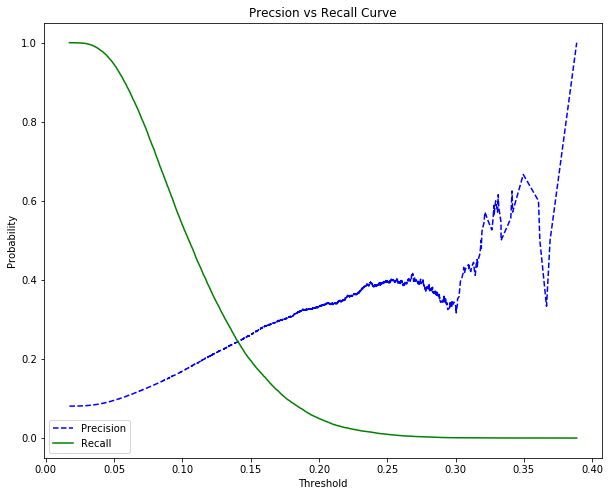
\includegraphics[scale = 0.7]{images/pic2.png}
    \caption{Precision và Recall với ngưỡng thay đổi.}
    \label{fig:PR}
\end{figure}
Nhìn vào ví dụ ta có thể thấy khi Precision cao thì Recall thấp, và ngược lại. Tức là ta rất khó để đánh giá đâu là mô hình tốt khi Precision cao hoặc Recall cao.
\subsubsection{F1 - score}
$F1$ Score là trung bình điều hòa giữa Precision và Recall. Do đó nó đại diện hơn trong việc đánh giá độ chính xác trên đồng thời Precision và Recall.
\begin{center}
    \[F1 = \frac{2}{\frac{1}{precision}+\frac{1}{recall}} = \frac{2*precision*recall}{precision+recall} \]
\end{center}
$F1$ có giá trị nằm trong khoảng $(0,1)$. Khi giá trị $F1$ score càng cao, tức mô hình phân loại của ta đang thực sự tốt. Trường hợp $F1 = 1$ tức là trường hợp mô hình đang hoạt động tốt nhất khi cả Precision và Recall đều bằng 1.\\
Khi mà precision và recall quá chênh lệch nhau thì  $F1$ score sẽ cân bằng được cả hai độ lớn này và giúp ta đưa ra một đánh giá khách quan hơn. 